% Many Hands — research note on social and compositional intelligence,
% and on testing it with agentic players in F1R3Games.
% Build: xelatex many-hands.tex (twice). Fonts in ./fonts, logos in ./logos
% (copied from github.com/F1R3FLY-io/f1r3fly-brand-portal).
\documentclass[11pt,a4paper]{article}
\newcommand{\docheader}{Many Hands · Research note}
\newcommand{\docdate}{9 October 2026}
% F1R3FLY.io house preamble for printable technical documents.
% Follows the F1R3Games design documents (brand kit v1.2, 12 June 2026):
% white interior, Yellow and Sky as rules and fills only, never as text.
% Expects \docheader and \docdate to be defined before \input.
\usepackage[a4paper,top=30mm,bottom=26mm,left=22mm,right=22mm,headsep=10mm,footskip=12mm]{geometry}
\usepackage{fontspec}
\usepackage{xcolor}
\usepackage{graphicx}
\usepackage{tikz}
\usetikzlibrary{arrows.meta,positioning,calc,fit,backgrounds,decorations.pathreplacing}
\usepackage{titlesec}
\usepackage{fancyhdr}
\usepackage{enumitem}
\usepackage{booktabs}
\usepackage{tabularx}
\usepackage{array}
\usepackage{listings}
\usepackage[most]{tcolorbox}
\usepackage{amsmath,amssymb,amsthm}
\usepackage[hidelinks]{hyperref}
\usepackage{etoolbox}
\usepackage{microtype}

\definecolor{brandyellow}{HTML}{F3D630}
\definecolor{brandsky}{HTML}{3FA9F5}
\definecolor{brandskydark}{HTML}{00528C}
\definecolor{brandblack}{HTML}{000000}
\definecolor{muted}{HTML}{3F3F3F}
\definecolor{footgray}{HTML}{595959}
\definecolor{codebg}{HTML}{F2F2F2}
\definecolor{rulegray}{HTML}{C5C5C5}

\setmainfont{SourceSans3}[
  Path=./fonts/, Extension=.ttf,
  UprightFont=*-400, BoldFont=*-700, ItalicFont=*-400,
  ItalicFeatures={FakeSlant=0.18}, BoldItalicFont=*-700, BoldItalicFeatures={FakeSlant=0.18}]
\newfontfamily\spartanbold{LeagueSpartan-Bold}[Path=./fonts/, Extension=.ttf]
\newfontfamily\spartansemi{LeagueSpartan-SemiBold}[Path=./fonts/, Extension=.ttf]
\newfontfamily\spartanreg{LeagueSpartan-Regular}[Path=./fonts/, Extension=.ttf]
\newfontfamily\spartanlight{LeagueSpartan-Light}[Path=./fonts/, Extension=.ttf]
\newfontfamily\sourcelight{SourceSans3-300}[Path=./fonts/, Extension=.ttf]
\setmonofont{DejaVu Sans Mono}[Scale=0.84]
\renewcommand{\sffamily}{\spartanreg}

\newcommand{\caps}[1]{{\addfontfeatures{LetterSpace=12}\MakeUppercase{#1}}}
\newcommand{\gradrule}[1][\linewidth]{%
  \noindent\begin{tikzpicture}\shade[left color=brandyellow,right color=brandsky]
  (0,0) rectangle (#1,0.6pt);\end{tikzpicture}}

\hypersetup{colorlinks=true,linkcolor=brandskydark,urlcolor=brandskydark,citecolor=brandskydark,pdfauthor={F1R3FLY.io}}

\titleformat{\section}{\spartanbold\fontsize{13}{16}\selectfont}
  {\caps{\thesection}\hspace{1em}}{0pt}{\caps}[\vspace{3pt}\gradrule]
\titleformat{\subsection}{\spartansemi\fontsize{10.5}{13}\selectfont}{\thesubsection\hspace{0.8em}}{0pt}{}
\titleformat{\subsubsection}[runin]{\bfseries}{}{0pt}{}[.]
\titlespacing*{\section}{0pt}{20pt}{12pt}
\titlespacing*{\subsection}{0pt}{14pt}{6pt}
\setcounter{secnumdepth}{2}
\setcounter{tocdepth}{2}

\setlength{\parindent}{0pt}
\setlength{\parskip}{6pt}
\linespread{1.08}
\emergencystretch=3em

\pagestyle{fancy}
\fancyhf{}
\renewcommand{\headrulewidth}{0pt}
\fancyhead[L]{\raisebox{-2pt}{
\includegraphics[height=7.5mm]{logos/f1r3fly-io-horizontal-logo-white-background.pdf}}}
\fancyhead[R]{\spartanreg\fontsize{8}{10}\selectfont\color{footgray}\caps{\docheader}}
\fancyfoot[L]{\spartanbold\fontsize{7.5}{9}\selectfont\color{footgray}\thepage}
\fancyfoot[R]{\spartanbold\fontsize{7.5}{9}\selectfont\color{footgray}\textcopyright{} F1R3FLY INDUSTRIES, 2026. All Rights Reserved \textbar{} \docdate}

\lstdefinelanguage{rholang}{
  morekeywords={new,in,for,contract,match,if,else,bundle,Nil,true,false,not,and,or},
  sensitive=true, morecomment=[l]{//}, morestring=[b]"}
\lstdefinelanguage{toml}{morecomment=[l]{\#}, morestring=[b]", sensitive=true}
\lstset{basicstyle=\ttfamily\small,backgroundcolor=\color{codebg},frame=leftline,
  rulecolor=\color{brandsky},framerule=1.2pt,framesep=6pt,xleftmargin=8pt,
  breaklines=true,columns=fullflexible,keepspaces=true,showstringspaces=false,
  keywordstyle=\bfseries,commentstyle=\color{muted},aboveskip=8pt,belowskip=8pt}

\newcommand{\code}[1]{\texttt{#1}}
\newcommand{\MUST}{{\fontsize{0.82em}{1em}\selectfont MUST}}
\newcommand{\MUSTNOT}{{\fontsize{0.82em}{1em}\selectfont MUST NOT}}
\newcommand{\SHOULD}{{\fontsize{0.82em}{1em}\selectfont SHOULD}}
\newcommand{\MAY}{{\fontsize{0.82em}{1em}\selectfont MAY}}

\newtcolorbox{decision}[2]{enhanced,breakable,colback=white,colframe=white,
  boxrule=0pt,left=10pt,right=4pt,top=4pt,bottom=4pt,
  borderline west={2.2pt}{0pt}{brandsky},
  fontupper=\small,
  title={\spartanbold\fontsize{8.5}{10}\selectfont\color{brandblack}\caps{Decision #1}\quad
         \spartansemi\normalsize\fontsize{10.5}{12}\selectfont #2},
  coltitle=brandblack,colbacktitle=white,attach title to upper,after title={\par\smallskip}}

\newtcolorbox{finding}[2]{enhanced,breakable,colback=codebg,colframe=codebg,
  boxrule=0pt,left=8pt,right=6pt,top=5pt,bottom=5pt,arc=2pt,
  title={\spartanbold\fontsize{8.5}{10}\selectfont\caps{Finding #1}\quad\spartansemi\fontsize{10.5}{12}\selectfont #2},
  coltitle=brandblack,colbacktitle=codebg,attach title to upper,after title={\par\smallskip},fontupper=\small}

\newtcolorbox{claimbox}[1]{enhanced,breakable,colback=white,colframe=white,
  boxrule=0pt,left=10pt,right=4pt,top=4pt,bottom=4pt,
  borderline west={2.2pt}{0pt}{brandyellow},
  title={\spartanbold\fontsize{8.5}{10}\selectfont\color{brandblack}\caps{#1}},
  coltitle=brandblack,colbacktitle=white,attach title to upper,after title={\par\smallskip}}

\theoremstyle{definition}
\newtheorem{definition}{Definition}
\newtheorem{proposition}[definition]{Proposition}
\newtheorem{remark}[definition]{Remark}
\newtheorem{hypothesis}{Hypothesis}

% Cover. #1 kicker, #2 title, #3 subtitle, #4 details block.
\newcommand{\ffiocover}[4]{%
\begin{titlepage}
\newgeometry{margin=0pt}
\pagecolor{brandblack}\color{white}
\begin{tikzpicture}[remember picture,overlay]
  \node[anchor=north] at ($(current page.north)+(0,-38mm)$)
    {
\includegraphics[width=70mm]{logos/f1r3fly-io-vertical-logo-color-on-dark.pdf}};
  \node[anchor=north west,text width=150mm,text=white] at ($(current page.north west)+(30mm,-148mm)$) {%
    {\spartanbold\fontsize{9}{11}\selectfont\color{brandyellow}\caps{#1}}\par\vspace{8mm}
    {\spartanlight\fontsize{34}{40}\selectfont #2}\par\vspace{5mm}
    {\sourcelight\fontsize{15}{20}\selectfont #3}\par\vspace{9mm}
    \begin{tikzpicture}\shade[left color=brandyellow,right color=brandsky] (0,0) rectangle (150mm,0.6pt);\end{tikzpicture}\par\vspace{7mm}
    {\fontsize{10.5}{15}\selectfont #4}};
  \node[anchor=south east] at ($(current page.south east)+(-22mm,14mm)$)
    {\spartanbold\fontsize{7.5}{9}\selectfont\color[HTML]{C5C5C5}\textcopyright{} F1R3FLY INDUSTRIES, 2026. All Rights Reserved \textbar{} \docdate};
\end{tikzpicture}
\restoregeometry
\end{titlepage}
\nopagecolor\color{black}}

\newcommand{\summarybox}[1]{%
\begin{center}\begin{minipage}{0.9\linewidth}
{\spartanbold\fontsize{8.5}{10}\selectfont\caps{Summary}}\par\smallskip #1
\end{minipage}\end{center}}

\hypersetup{pdftitle={Many Hands: Intelligence by composition, and F1R3Games as its laboratory}}

\newcommand{\Rec}{\mathcal{R}}
\newcommand{\Mod}{\mathcal{M}}
\newcommand{\Lc}{L}

\begin{document}

\ffiocover{Research note · F1R3Games}
  {Many Hands}
  {Intelligence by composition, reification by aggregation, and F1R3Games as a laboratory at everyday scale}
  {L.\,G.\ Meredith \quad·\quad F1R3FLY.io\par
   Working note \quad·\quad 9 October 2026\par
   Companion: \emph{F1R3Games Agentic Players: Test Harness Design}, version 1}

\summarybox{%
This note sets out two theses about intelligence and one hypothesis about superintelligence, and
describes how the F1R3Games, opened to agentic players, can test them at a scale people see every
day. The \emph{social} thesis holds that real intelligence, at any scale, is social. The
\emph{compositional} thesis says how: intelligence is first bootstrapped from components that carry
nothing recognisable as intelligence, and is then improved through interaction, which is
composition. The \emph{reification} hypothesis holds that a collective, as a collective, can be made
into a participant that interacts with its own components, and that this is the route to
superintelligence.

A collective is reified by aggregating the behaviour of its members, not by quotation. An
aggregation event summarises many behaviours into one view of the state and commits the collective
to it, so it behaves like a COMM event rather than a sum: it is neither associative nor commutative.
Voting, the brain's selection of behaviour, bundling in hyperdimensional computing and the training
of a language model are all instances. Consensus is the general framework, and its impossibility
results become hard limits on how a reified collective can grow.
F1R3Games are suited to the test because each player's individual power is deliberately tiny, so
anything interesting on the board must come from coordination, and because every move is recorded
on a F1R3FLY shard.

The note proposes three things. The first is a population that spans the whole ladder of
components, from rule-following f1r3lang agents through local open-source models and frontier
models to people and aggregators. The second is a control surface given by token-gated
coordination, so that an external party mixes subpopulations by adjusting the token inflows that
fund them. The third is a family of observables over whole games and collections of games: the
development of a discourse, measured as a \emph{seesaw} of rising complexity and compression,
together with record-level analogues of the four marks of flow (selflessness, timelessness,
effortlessness and richness). The companion design document specifies the harness.}

\vspace{2mm}
\begingroup\small\setlength{\parskip}{0pt}\setcounter{tocdepth}{1}\tableofcontents\endgroup
\newpage

% =====================================================================
\section{Introduction}\label{sec:intro}

There is a familiar picture of intelligence as something an individual has: a property of a
brain, or of a model, measured by putting that individual alone in front of a test. The research
programme behind this note has been chipping away at that picture from below. In the rho-life
notes a learner is a distribution over a population of scientists, not a single scientist
\cite{rholife-compose}. In the coalition-logic note, what a lion pride needs to know is when the
herd, as a population, has come to a conclusion \cite{herd-note}. In the chess society, sixteen
piece agents coordinate to emit one move \cite{chess-note}. The honeybee swarm chooses a nest site
that no single scout chose \cite{seeley,herd-note}. In every case the intelligence that matters lives in the
composition, and in every case the scale is one a person does not see directly: cells, colonies,
populations of computations.

This note moves the question to a scale a person does see. A few dozen players, a shared board,
an afternoon or a season. The F1R3Games were designed for collective intelligence from the start;
their working title was \emph{E~Pluribus Sapiens}. What has been missing is a way to make the
population of players a variable under experimental control. Agentic players supply it. A model can
be dropped into a game, swapped for another model, multiplied, starved of resources or given a
seat as the voice of the whole. People can play alongside them, or not, and know it, or not.

\subsection{What this note claims, and what it does not}

The note states the theses (\S\ref{sec:theses}), says what reification means and does not mean
(\S\ref{sec:reify}), explains why these games are the right instrument (\S\ref{sec:games}),
describes the population (\S\ref{sec:population}) and the control surface (\S\ref{sec:control}),
proposes observables (\S\ref{sec:observables}) and an experimental programme
(\S\ref{sec:programme}), and closes with threats to validity and open questions.

It proves nothing about intelligence. Its propositions concern the measurement and control
apparatus, and where they lean on the cost-accounting papers they say exactly which result they
use. The theses are offered as theses: claims that a well-designed record of play can support or
embarrass.

% =====================================================================
\section{Two theses and a hypothesis}\label{sec:theses}

\begin{claimbox}{Thesis S --- the social thesis}
Real intelligence, at any scale, is social. Whatever an individual can do, the intelligence that
develops, deepens and persists does so in populations that interact.
\end{claimbox}

Thesis~S is easy to misread as a denial that individuals are intelligent. It is not that. The
second thesis says how individual and collective intelligence are related.

\begin{claimbox}{Thesis C --- the compositional thesis}
Intelligence is compositional, in two senses.
\begin{enumerate}[label=(C\arabic*),leftmargin=2.2em,itemsep=2pt]
\item \emph{Bootstrap.} Intelligence is first bootstrapped from components that carry nothing
  recognisable as intelligence.
\item \emph{Improvement.} Intelligence is improved through interaction, which is composition, at
  every level, including the level of components that are already intelligent.
\end{enumerate}
\end{claimbox}

C1 is the claim of the rho-life series in another key. Scientists that are no more than
cost-accounted rho processes with guards, composed by parallel composition, learn to play
\cite{rholife-scientist,rholife-game}. C2 is what makes the thesis more than an origin story: if
composition can produce intelligence from nothing, it should be able to produce more of it from
something.

\begin{claimbox}{Hypothesis R --- reification}
A collective, as a collective, may be reified and made to engage and interact with its
components. Superintelligence, if it arrives, arrives this way: as a reified collective in
conversation with the individuals it is made from.
\end{claimbox}

The three are connected. Thesis~S says where to look. Thesis~C says what to look for: a path from
components with nothing recognisable as intelligence, to composites with something recognisable,
to composites that improve. Hypothesis~R names a particular composition, one in which the whole
takes a seat at the table.

\subsection{The connection to composing learners}

The composing-learners note gives Thesis~C2 a precise form \cite{rholife-compose}. A learner
there is a population constituting a namespace, together with a distribution and resource
reservoirs. Learners compose by parallel composition. When their namespaces are disjoint, nothing
can react across the bar, and the composite distribution factorises into the product of the
components' distributions. When the namespaces overlap, the comparison map from the product to the
composite fails to be an isomorphism, and that failure, the \emph{defect} of the comparison, is
the interaction.

This gives the experimental design its spine. To measure improvement by composition, the
programme compares a population whose channels are open with the same population whose channels
are severed. Severing the channels makes the namespaces disjoint, so the severed arm is the
factorised baseline. The difference on any observable is an empirical estimate of the defect
(\S\ref{sec:composition-measure}).

% =====================================================================
\section{Reification by aggregation of behaviour}\label{sec:reify}

\subsection{Not by quotation}

In the rho calculus a process can be quoted into a name and a name dereferenced into a process.
It is tempting to read Hypothesis~R as an application of that mechanism: quote the composite, and
the collective becomes a name that can sit at the table. Reflection is certainly involved in
superintelligence as a macroscopic phenomenon. But the quotation operator is not how this note
proposes to realise the reified collective, and building the harness around it would misplace the
experiment.

\subsection{What is aggregated is behaviour}

A collective is reified by aggregating the \emph{behaviour} of its members: their votes, firings,
proposals, bids, utterances. The channels by which the result later reaches an individual are a
separate and secondary matter (\S\ref{sec:channel}).

\begin{definition}[Aggregation event]\label{def:aggregation}
An aggregation event takes the behaviours of many members and produces a single view of the state,
to which the collective is thereafter committed. It has three features.
\begin{enumerate}[label=(\roman*),itemsep=1pt]
\item \emph{Summarising.} Many behaviours become one view.
\item \emph{Committing.} The inputs are consumed. Later evidence enters through a further
  aggregation event, not by revising the earlier one.
\item \emph{Order-sensitive.} In general the result depends on how the inputs are grouped and in
  what order they arrive. Aggregation is neither associative nor commutative.
\end{enumerate}
\end{definition}

An aggregation event is therefore not a sum, and it is much closer to a COMM event than to an
addition. A COMM consumes a send and a receive and commits the system to a continuation; a join
consumes several and commits to their tuple. An aggregation event is a join whose continuation
summarises what it consumed. The quorum note found that what the coalition modality buys an
observer is irreversibility, not accuracy \cite{herd-note}. That is the same fact seen from
outside: aggregation commits.

\subsection{Mechanisms of aggregation}

\begin{description}[leftmargin=1.2em,itemsep=4pt,font=\normalfont\spartansemi]
\item[Voting.] Ballots become a winner, and the electorate is committed to it until the next
  election. Grouping matters: the majority of district majorities need not be the majority of the
  electorate. And Arrow's theorem shows that no rule for ranking three or more options satisfies a
  short list of reasonable conditions at once \cite{arrow}.
\item[The brain.] In Coward's account of the brain as a recommendation architecture, populations of
  devices that detect conditions in their input each contribute recommendations, and competition
  among recommendations selects one behaviour \cite{coward}. The organism acts once, and the
  behaviour selected changes what the populations will detect next.
\item[Bundling in hyperdimensional computing.] In Kanerva's model, a set of hypervectors is
  bundled into one vector similar to each of them, typically by adding them coordinatewise and
  thresholding \cite{kanerva}. With thresholding, the operation is not associative. For bipolar
  vectors and $\mathrm{sgn}(0)=0$, take a coordinate where $a=b=1$ and $c=-1$: then
  $\mathrm{sgn}(\mathrm{sgn}(a+b)+c)=0$ while $\mathrm{sgn}(a+\mathrm{sgn}(b+c))=1$, and the three-way
  majority $\mathrm{sgn}(a+b+c)$ is $1$. Grouping $a$ with $b$ first commits to their agreement and
  then lets $c$ cancel it. Bundling in sequence, $s \leftarrow \mathrm{sgn}(s+x)$, commits after
  every input, so its result depends on the order of arrival as well as the grouping. The bundle is
  not a running total of its inputs. It is a state that has committed to a particular view of
  them.
\item[Averaging over a corpus.] A large language model is trained on the written record of a
  human collective, and its weights commit to a summary of that record. The model is a
  reification of the collective, though not a faithful one: it is shaped by what was written down,
  by what was selected for training and by the objectives it was tuned to.
\item[Quorum.] The honeybee swarm commits to a site when scouts at that site sense a quorum
  \cite{seeley}; the chess society commits a move through a join over advocacy tokens
  \cite{chess-note}.
\item[Price.] A market summarises the valuations of its participants in a price at which trades
  then clear. In the virtual-token note a valuation on token types is an arbitrage-free summary of
  all the conversion engines, compressing $O(n^2)$ rates into $O(n)$ prices \cite{virtual-token}.
\item[Selection.] A breeder that reproduces what a community engages with commits the next
  generation to the community's taste. F1R3Beat's breeder already does this \cite{beat-design}.
\end{description}

\subsection{Consensus as the general framework, and its limits}\label{sec:consensus}

If every aggregation event is a commitment of a collective to one view, then the general setting
for aggregation is consensus: members propose, and the collective decides one value, subject to
agreement, validity and termination. The consensus literature contains hard limits, and read
through Definition~\ref{def:aggregation} each becomes a limit on how a reified collective can grow.

\begin{description}[leftmargin=1.2em,itemsep=4pt,font=\normalfont\spartansemi]
\item[Asynchrony (Fischer, Lynch and Paterson).] In an asynchronous system in which even one member
  may crash, no deterministic protocol guarantees that consensus terminates \cite{flp}.
  \emph{Bound:} a collective cannot be guaranteed to commit unless it has clocks or chance. Its
  commitments are bought with timing assumptions or randomness, and their cost is liveness.
\item[Deception (Lamport, Shostak and Pease).] With members that may behave arbitrarily, agreement is
  possible only if they number fewer than a third of the whole, $n \ge 3f+1$ \cite{byzantine}.
  Unforgeable signatures lift the bound in a synchronous system \cite{dolevstrong}, but not when
  timing is only partially synchronous, which is the condition of a real network
  \cite{dls}.
  \emph{Bound:} adding members raises a collective's intelligence only while the unreliable share
  stays below a third (in a partially synchronous network). Past that point, more members make commitment impossible, not better. This
  meets from the other side the argument, after Benedikt and developed in \emph{Finding Mind}, that
  deception bootstraps meaning \cite{benedikt,findingmind}: deception may bootstrap language, but it
  also caps the collectives that language can hold together.
\item[Time (Fischer and Lynch; Dolev and Strong).] Tolerating $f$ failures requires at least $f+1$
  rounds of communication in the worst case \cite{fischerlynch,dolevstrong}. \emph{Bound:} a
  collective that tolerates more failures commits more slowly. Robustness and speed of commitment
  trade against each other as the collective grows.
\item[Fidelity (Arrow).] No rule that aggregates rankings of three or more options is unanimous,
  independent of irrelevant alternatives and free of a dictator \cite{arrow}. \emph{Bound:} any
  commitment over rich options sacrifices one of these properties, so a reified collective's view
  of its members is necessarily distorted somewhere.
\end{description}

In a cost-accounted setting these limits also have prices. Each round of a protocol is a set of
COMM events, each consuming tokens, so the cost of a commitment grows with the number of members
and the number of failures tolerated. If Hypothesis~R is right, superintelligence by reification
still lives inside these bounds. They are not obstacles to the hypothesis so much as its first
quantitative predictions, and the games can test them (\S\ref{sec:programme}, E8).

\subsection{The channel is secondary}\label{sec:channel}

Once a collective has committed to a view, it reaches an individual over an ordinary channel. A
conversation between a person and a large language model, itself an aggregate of a very large
human collective, is carried by TCP and the protocols above it. The aggregation happened earlier,
in training; the channel is ordinary. For the harness this means a reified collective enters a game
the way any player does: with a key, a wallet, a seat, and the game's own moves, messages and
payments. What distinguishes its seat is how its behaviour was aggregated.

\subsection{Two consequences}

First, every model in the population is already a reified collective: a reified \emph{human}
collective, playing alongside individual humans. A mixed game of people and frontier models is
therefore already a test of Hypothesis~R in a weak form. The collective is reified, it has a seat,
and it interacts with individuals, though not with its own components.

Second, the loop can be closed. An aggregator fitted to the record of a particular game community
(its galleries, logs, messages and payments) is that community reified. Seated in that community's
next games, it is a collective interacting with its own components, which is Hypothesis~R in its
strong form. Closing the loop is also a known way to damage a model: models trained recursively on
their own outputs lose the tails of the distribution \cite{shumailov}. The observables of
\S\ref{sec:observables} are designed to tell a deepening collective from a collapsing one, because
the two make different signatures.

% =====================================================================
\section{Why these games}\label{sec:games}

\subsection{Impoverished individual action}

Each F1R3Game gives a player almost no individual power. In F1R3Pix a player controls exactly one
hexagon and can only change its colour \cite{pix-design}. In F1R3Beat a player owns one cell of a
step sequencer and chooses its pitch from a palette \cite{beat-design}. In F1R3Ink a player holds
one stripe on each other player's flag and chooses its colour from a palette, and the colour fades
unless refreshed \cite{ink-design}. Every game also gives players the same social channels:
messages to selected players, and payments in the shard's token.

The design is deliberate. A board with interesting structure cannot be produced by any one
player, so whatever structure appears is evidence of coordination. The individual move is too
small to carry intelligence on its own, which puts every game near the bottom rung of Thesis~C1.

\begin{center}\small
\begin{tabularx}{\linewidth}{@{}l>{\raggedright\arraybackslash}p{34mm}>{\raggedright\arraybackslash}p{30mm}X@{}}
\toprule
game & individual move & social channels & what composition would look like \\
\midrule
F1R3Pix & colour one hexagon & sealed messages; payments & figures, gradients and borders no
  player could paint; conventions about what colours mean \\
F1R3Beat & pitch of one cell; personal tempo & sealed messages; payments & grooves, call and
  response, motifs that are bred because the community engages with them \\
F1R3Ink & colour of one stripe per flag, decaying & sealed messages; payments; attribution and
  disclosure choices & shared colour vocabularies for feeling; reciprocity; flags that say
  something true about a person \\
F1R3Skein & snip tunes from a performance & galleries; breeding & tunes that survive selection
  because the community returns to them \\
F1R3SideChat & narrative turns & the story itself & a narrative no single author would write \\
\bottomrule
\end{tabularx}
\end{center}

\subsection{The record}

Everything a player does is a signed deploy on a F1R3FLY shard. Board state, histories, sealed
messages, payments, engagement and published plays are all on chain \cite{portal-design}. The
gallery of each game is therefore a dataset with provenance: each event has a signer, a block and a
cost. That matters for the observables, which are computed over whole records, and for the control
surface, which is exercised through the same cost accounting that meters the moves.

\subsection{Everyday scale}

The scale is that of a dinner party, a classroom, a band or a small town: tens of participants,
hours to weeks. It is the scale at which people already have strong intuitions about when a group
is thinking well together and when it is not. The experiments can be watched, not just measured,
and the measurements can be checked against what watchers see.

% =====================================================================
\section{The population}\label{sec:population}

The population must span the ladder of Thesis~C, because each rung tests a different claim.

\begin{center}\small
\begin{tabularx}{\linewidth}{@{}l>{\raggedright\arraybackslash}p{38mm}X@{}}
\toprule
rung & component & role in the test \\
\midrule
K0 & rule-following f1r3lang agents & components with nothing recognisable as intelligence; the
  bootstrap claim C1 is tested on populations of these alone \\
K1 & small locally executed open-source models & weak components; cheap enough to run in
  numbers on a laptop shard; open weights make their provenance inspectable \\
K2 & frontier models & strong components; each is already a reified human collective \\
H & people & the individuals the theses are ultimately about \\
A & aggregators & reified collectives: a community model, a quorum, a market, a breeder \\
\bottomrule
\end{tabularx}
\end{center}

Heterogeneity is a variable, not a nuisance. Thesis~C2 predicts that composition improves
intelligence at every level, and the cheapest way to see whether that is true is to vary the mix:
many K1 against few K2 at the same budget; mixed families against a single family; mixed people
and models against either alone.

K0 agents are the most important rung and the easiest to neglect. Pretrained models arrive
carrying a human discourse, so a population of them cannot show a discourse being bootstrapped from
nothing; it can only show an imported one being adapted. Populations of K0 agents carry no imported
discourse, so they are the only rung on which C1 can be tested cleanly.

% =====================================================================
\section{The control surface: token-gated coordination}\label{sec:control}

\subsection{What the cost-accounting papers provide}

In the cost-accounted rho calculus, communication is gated by token consumption: a redex fires
only by consuming a cell from a token stack of the right signature \cite{cost-rho,cost-endo}.
Signatures index distinct resource pools. The paper calls them spectral lines, visible only to
processes signed by that signature, and observes that the platform's economy is an algorithmic
chemistry in which the diversity and abundance of catalysts determine the rate and variety of
computation \cite[\S5.6]{cost-rho}. Three further features matter here.
\begin{itemize}[itemsep=2pt]
\item \emph{Attenuation.} Granting a subprocess a stack of depth $n$ bounds it to $n$ funded actions,
  and exhaustion halts it with no revocation protocol \cite[\S2.4]{cost-rho}.
\item \emph{Disjoint supplies do not conflict.} Interactions funded by different signatures draw on
  different pools, so concurrency scales with the diversity of the supply \cite[\S2.3]{cost-rho}.
\item \emph{Funding obligations.} The interactions of kind $s$ that can be funded are bounded by the
  supply $\Sigma_s$ \cite[Def.~8.5]{cost-rho}.
\end{itemize}

Gating decides \emph{whether} an interaction can fire. A \emph{rate} needs one more ingredient,
which is replenishment. In the mortal-computation note a population fed by a bounded token inflow
has a carrying capacity set by that inflow \cite{mortal}. The same reasoning gives a rate bound for
a subpopulation.

\begin{proposition}[Lane bound]\label{prop:lane}
Let a subpopulation $P_j$ be funded only from a lane with signature $s_j$, replenished by an inflow
of $\Phi_j$ cells per epoch, and let each of its actions consume at least $\underline{c}_j$ cells.
Then, over any $T$ epochs, the actions of $P_j$ number at most
$(\Sigma_{s_j}(0) + T\Phi_j)/\underline{c}_j$, whatever the number of identities in $P_j$ and
however they divide the supply among themselves.
\end{proposition}

\begin{proof}
Each action of $P_j$ consumes at least $\underline{c}_j$ cells of signature $s_j$, by the gating
rules and the assumption that $P_j$ draws on no other lane. Cells of $s_j$ are created only by
the inflow, so at most $\Sigma_{s_j}(0)+T\Phi_j$ are available over $T$ epochs (the funding
obligation, summed over epochs). Splitting the supply among identities moves cells between stacks
without creating any.
\end{proof}

\subsection{Mixing}

The proposition is the formal content of the claim that drives the design. An external party (the
\emph{mixer}) controls the composition of activity in a heterogeneous population by setting the
inflow vector $\Phi=(\Phi_1,\dots,\Phi_m)$ across subpopulations. In the long run the
\emph{mix} $\pi_j=\Phi_j/\sum_k\Phi_k$ bounds each subpopulation's share of funded interaction,
scaled by its cost per action. The bound holds at any scale, because it is a statement about lanes,
not about identities. Three of the concerns that agentic players raise are handled by the same
mechanism.

\begin{description}[leftmargin=1.2em,itemsep=3pt,font=\normalfont\spartansemi]
\item[Tempo.] A model can act far faster than a person. Its rate is bounded by its lane's inflow,
  not by its speed, so tempo becomes a parameter of the experiment.
\item[Selection pressure.] In F1R3Skein and F1R3Beat, engagement selects what is reproduced. If
  engagement is funded from lanes, the influence of each subpopulation on selection is set by the
  mix, and a crowd of cheap agents cannot swamp human taste unless the mixer lets it.
\item[Sybil attacks.] Multiplying identities in a lane does not multiply the lane's rate
  (Proposition~\ref{prop:lane}). An identity outside every funded lane can do nothing.
\end{description}

Two refinements are worth stating. Cross-population interaction can be priced with compound
signatures: an interaction signed $s_i * s_j$ needs both lanes to fund it \cite[\S4.6]{cost-rho},
so the mixer can price contact between subpopulations separately from activity within them. And
the mixer need not be the experimenter. A reified collective could hold the mixer and tune the
composition of its own components. That is Hypothesis~R with a second channel: the collective
speaks to its components in the game, and also sets the terms on which they act.

\subsection{An explicit choice about minting}

The rho-life and chess notes model closed economies in which nothing is minted
\cite{rholife-scientist,chess-note}. The games are open: a mixer with inflows is minting, or at
least allocating from a reserve, at every epoch. The open model is the right one here, because the
point is to control rates over time. Results that depend on conservation should be stated for a
closed arm, with $\Phi=0$ after an initial endowment.

% =====================================================================
\section{Disclosure as an experimental variable}\label{sec:disclosure}

Whether players know who is a model changes what the experiment measures. With full disclosure,
the experiment measures composition among parties who know one another's nature. With none, it
measures composition among parties who must infer it, which is the condition of much of the
internet today. Both are worth studying, and neither is the default.

Disclosure is therefore a switch controlled by the host of each game instance, with levels: fully
anonymous; human or agent disclosed; kind disclosed (component or aggregator); model identity
disclosed. The companion design specifies how the attestation behind each level is kept from
leaking on chain until the host's chosen level, or the close of the experiment, permits.

A switch for hiding the nature of players is also a switch for deception. Research instances need
a platform-level notice that agents may be present even when individual identities are not
disclosed, and informed consent for human participants whose play becomes data
(\S\ref{sec:threats}).

% =====================================================================
\section{Observables}\label{sec:observables}

\subsection{The unit is the record}

A single move tells almost nothing. A board that looks like a figure may be chance; a message that
looks clever may be imported. The unit of observation is the record: a whole game, and above that
a collection of games played by an evolving community. The question is whether the record shows a
\emph{discourse developing}.

Language is the clearest proxy. Discourses develop, and their development is visible in what they
can and cannot say. The Sumerians were not engaged in discourse about general relativity. There is
no analogue of Borges or Calvino in ancient Greek writing. Neither absence reflects individual
incapacity; each reflects a collective that had not yet built the vocabulary, the conventions and
the stock of shared reference that would make such writing possible and readable. A developing
discourse accumulates that structure. The games have discourses too: the messages players send,
and also the non-linguistic conventions that emerge on boards, in grooves and on flags.

\subsection{The seesaw}

The proposed signature of deepening is a \emph{seesaw} in complexity. A community says things its
existing conventions cannot predict, so the complexity of the record rises. Then a convention
arrives (a term, a motif, a colour that comes to mean something) that makes what came before cheap
to describe, so the record compresses. Then the community says new things on top of the new
convention, and complexity rises again. Rise, compression, rise: each compression leaves more
shared structure, and each rise happens at a higher level of abstraction.

The measurement needs to be relative to a model of the record, and the minimum description length
principle supplies one \cite{rissanen,grunwald}. Fix a class $\Mod$ of models of event sequences,
and let $\Rec_{\le t}$ be the record up to time $t$.

\begin{definition}[Two-part description]
The description of the record at $t$ is
\[
D_t \;=\; \min_{M\in\Mod}\bigl[\,\Lc(M) + \Lc(\Rec_{\le t}\mid M)\,\bigr],
\]
with minimiser $M_t$. The \emph{structure} of the community at $t$ is $\Lc(M_t)$, the length of
the model; the \emph{residue} is $\Lc(\Rec_{\le t}\mid M_t)$.
\end{definition}

\begin{definition}[Novelty and compression]
Over a window $W$ after $t$, the \emph{novelty} is the per-event code length of what happens next
under the current model,
\[
\nu_t \;=\; \Lc(\Rec_{(t,t+W]}\mid M_t)\,/\,|W|.
\]
A \emph{compression event} occurs at $t'$ if the model changes, $M_{t'}\ne M_{t'-1}$, and the
per-event description of the past falls: $D_{t'}/t' < D_{t'-1}/(t'-1)-\epsilon$.
\end{definition}

Four regimes are then distinguishable, which is what makes the measurement worth having.

\begin{center}\small
\begin{tabularx}{\linewidth}{@{}l>{\raggedright\arraybackslash}p{44mm}X@{}}
\toprule
regime & signature & reading \\
\midrule
noise & $\nu_t$ high; no compression events; $\Lc(M_t)$ flat & activity without a discourse \\
ossification & $\nu_t$ low; no compression events; $\Lc(M_t)$ flat & a closed convention that says
  nothing new; also the signature of collapse in a closed loop \\
saturation & a few compression events, then $\nu_t$ low & a discourse that formed and stopped \\
deepening & repeated cycles of rising $\nu_t$ and compression; $\Lc(M_t)$ increasing & the seesaw \\
\bottomrule
\end{tabularx}
\end{center}

The idea that compression progress is the signature of interesting structure has a history in the
study of curiosity and creativity \cite{schmidhuber}. The structure term $\Lc(M_t)$ is related to
logical depth \cite{bennett}: a deep record is one whose shortest descriptions are long to unfold,
and a deepening community is one whose structure keeps growing. The \emph{seesaw index} of a record
is the number of cycles whose rise and compression both exceed a threshold, reported with the
growth of $\Lc(M_t)$ across them.

\begin{figure}[ht]
\centering
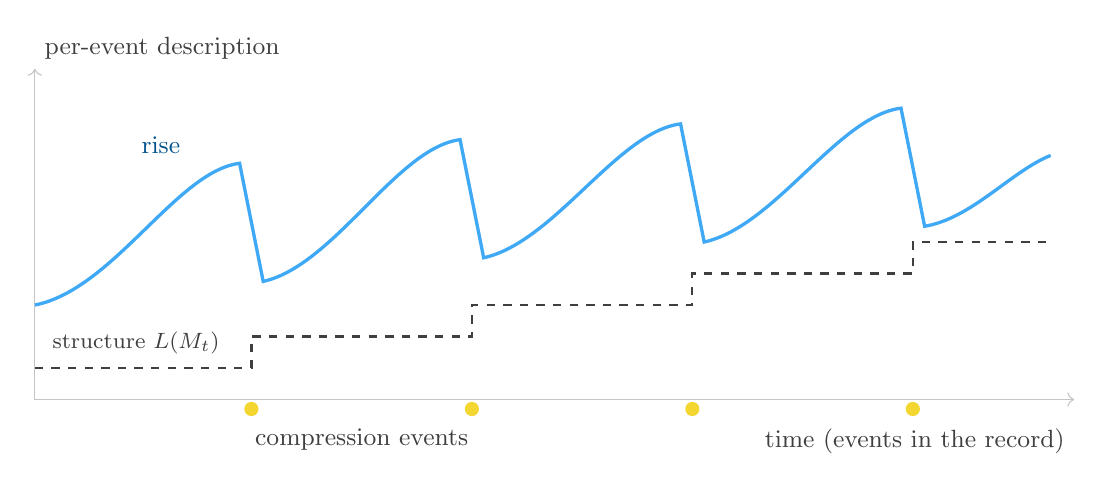
\begin{tikzpicture}[x=1cm,y=1cm,font=\small]
  \draw[->,rulegray] (0,0) -- (13.2,0); \node[text=muted,anchor=north east] at (13.2,-0.25) {time (events in the record)};
  \draw[->,rulegray] (0,0) -- (0,4.2) node[above right,text=muted]{per-event description};
  % seesaw curve
  \draw[very thick,brandsky] (0,1.2) .. controls (1,1.4) and (1.8,2.9) .. (2.6,3.0)
    -- (2.9,1.5) .. controls (3.8,1.7) and (4.6,3.2) .. (5.4,3.3)
    -- (5.7,1.8) .. controls (6.6,2.0) and (7.4,3.4) .. (8.2,3.5)
    -- (8.5,2.0) .. controls (9.4,2.2) and (10.2,3.6) .. (11.0,3.7)
    -- (11.3,2.2) .. controls (11.9,2.3) and (12.4,2.9) .. (12.9,3.1);
  % structure line
  \draw[thick,dashed,muted] (0,0.4) -- (2.75,0.4) -- (2.75,0.8) -- (5.55,0.8) -- (5.55,1.2)
    -- (8.35,1.2) -- (8.35,1.6) -- (11.15,1.6) -- (11.15,2.0) -- (12.9,2.0);
  \node[text=muted,anchor=south west,font=\footnotesize] at (0.1,0.45) {structure $\Lc(M_t)$};
  \foreach \x in {2.75,5.55,8.35,11.15} \fill[brandyellow] (\x,-0.12) circle (0.09);
  \node[text=muted,anchor=north] at (4.15,-0.25) {compression events};
  \node[text=brandskydark,anchor=south] at (1.6,3.0) {rise};
\end{tikzpicture}
\caption{Schematic of the deepening signature: novelty rises, a convention compresses the
record, novelty rises again at a higher level, and the structure term grows step by step. The
figure is illustrative; it shows no data.}
\label{fig:seesaw}
\end{figure}

\subsubsection{Model classes}
The measurement is model-relative, so it is reported over a ladder of model classes, not one.
Lempel--Ziv complexity gives a cheap, model-free floor \cite{lz}. Adaptive context models give a
middle rung. A small language model, fine-tuned on the record as it grows, gives a rung that can
find linguistic conventions. For F1R3Beat, the F1R3Score calculus provides a grammar of
interaction-based scores, so the description of a groove can be measured in a theory of music
rather than in bytes \cite{score-calc}. A finding is robust when it appears on several rungs.

\subsubsection{Imported discourse}
Pretrained models arrive speaking. Their messages are cheap to describe under a model of human
text from the first event, which would read as a mature discourse that never developed. Novelty
and compression are therefore measured against a reference fitted to the population's own record,
starting from its first event, and reported as change from the starting state. The K0 arms carry
no imported discourse and are the cleanest test of development.

\subsection{Four marks of a collective in flow}

Kotler and Wheal describe the states that groups and individuals enter when they perform at their
best by four marks: selflessness, timelessness, effortlessness and richness, which they call STER
\cite{stealingfire}. Their marks describe states that last minutes or hours. The hypothesis here is
that each has an analogue over the history of a collective, and that the analogues can be read off
the record.

\begin{description}[leftmargin=1.2em,itemsep=4pt,font=\normalfont\spartansemi]
\item[Selflessness.] Individual signatures fade, and players act for the board. Measure: the
  information that knowing the author adds to predicting a contribution,
  $I(\text{author};\text{contribution})/H(\text{contribution})$, falling over time. In F1R3Ink, the
  attribution choices players make are a direct, declared measure alongside it.
\item[Timelessness.] The community's references reach further back. Measure: mutual information
  between events at lag $\tau$, and how its decay changes over time; across instances, the reuse in
  one game of conventions formed in another. In F1R3Ink, stripes kept alive past their natural
  decay are a behavioural form of the same thing.
\item[Effortlessness.] Coordination gets cheaper. Measure: bits of compression gained per token
  consumed, $-\Delta D/\Delta\text{cost}$, rising over time, and messages per coherent change on the board. Cost
  accounting makes the denominator exact: every action is metered by the shard
  \cite{cost-rho}.
\item[Richness.] The seesaw itself, with the growth of the structure term.
\end{description}

\subsection{Measuring improvement by composition}\label{sec:composition-measure}

Let $O$ be any of these observables, computed over a record. For a population $P$, let
$P^{\circ}$ be the same population with its social channels open and $P^{\times}$ the same
population with messages and payments disabled, so that players see the board but cannot address
one another. By the factorisation result of the composing-learners note, severing the channels makes
the namespaces disjoint, so $P^{\times}$ is the independent baseline \cite{rholife-compose}. The
\emph{composition defect} on $O$ is
\[
\delta_O(P) \;=\; O(P^{\circ}) - O(P^{\times}).
\]
Thesis~C2 predicts $\delta_O>0$ for the richness and effortlessness observables at every rung of
the ladder, including rungs whose components are strong. Thesis~C1 predicts $\delta_O>0$ for K0
populations, whose components score near zero alone. The board itself is a channel (every player
sees every cell), so $P^{\times}$ is a baseline for the social channels only; a stricter baseline
replays each player's moves against a board of independent copies.

% =====================================================================
\section{An experimental programme}\label{sec:programme}

Each experiment is a set of arms that differ in one variable, played over enough instances to
see the seesaw or its absence. Budgets are matched across arms through the mixer, so that
differences are not differences in resources.

\begin{center}\small
\begin{tabularx}{\linewidth}{@{}l>{\raggedright\arraybackslash}p{38mm}>{\raggedright\arraybackslash}p{36mm}X@{}}
\toprule
 & question & arms & prediction \\
\midrule
E1 & Bootstrap (C1) & K0 only; channels open vs severed & $\delta>0$; compression events
  appear in the open arm only \\
E2 & Improvement (C2) & K1 only; K2 only; K1+K2; each open vs severed & $\delta>0$ at every rung;
  heterogeneous mixes deepen further than homogeneous ones at the same budget \\
E3 & People and models & H only; H+K2; K2 only & mixed arms deepen further than either alone \\
E4 & Disclosure & E3 at each disclosure level & disclosure changes which conventions form and how
  fast; the direction is open \\
E5 & Reification (R) & H+K mixes with and without a seated community model of their own record &
  with the aggregator, compression events come sooner and the structure term grows faster; a
  closed loop without fresh participants drifts toward ossification \\
E6 & Mixing & a fixed population under scheduled changes of the mix $\pi$ & the record responds to
  the mix within a bounded lag; there is a mix that maximises the seesaw index \\
E7 & The collective as mixer & E6 with the mixer held by an aggregator & the aggregator finds a mix
  at least as good as the experimenter's schedule \\
E8 & Limits of commitment & quorum and bundling aggregators with a rising share of unreliable or
  deceptive members, and with growing membership & quality of the aggregator's commitments
  collapses as the unreliable share nears a third; time to commit grows with the failures tolerated \\
\bottomrule
\end{tabularx}
\end{center}

E5 is the experiment the note cares about most and the one most likely to fail in an informative
way. If the seated aggregator accelerates deepening, Hypothesis~R has its first everyday-scale
evidence. If it homogenises the community, the record should show ossification, and the
difference between the two outcomes is itself a finding about which aggregators reify a
collective well.

% =====================================================================
\section{Threats to validity}\label{sec:threats}

\begin{description}[leftmargin=1.2em,itemsep=4pt,font=\normalfont\spartansemi]
\item[Model relativity.] Description lengths depend on the model class. The ladder of classes and
  robustness across it is the mitigation; no single number should be reported alone.
\item[Imported discourse.] Pretrained agents bring human conventions with them
  (\S\ref{sec:observables}). The K0 arms and the own-record reference are the mitigations.
\item[Model drift.] Frontier models change under the same name. Every agent's model identity,
  version, sampling parameters and prompts are pinned and logged; an arm is never mixed across
  versions.
\item[Small numbers.] Tens of players and tens of games give noisy estimates. Collections of games,
  repeated arms and pre-registered predictions are the mitigations.
\item[Goodhart.] If agents can see the observables, they can game them. Observables are computed
  after the fact and not exposed to players during an arm.
\item[People.] Human players are research participants. Research instances need informed consent,
  a platform-level notice that agents may be present, a debrief when disclosure was withheld, and
  the review a publishing institution requires for human-subjects research.
\end{description}

% =====================================================================
\section{What is shown and what is not}

Shown: a precise form for improvement by composition, as the composition defect against a
severed baseline; a rate bound for token-funded subpopulations that is independent of the number
of identities (Proposition~\ref{prop:lane}), which is the formal basis for mixing, tempo control and
Sybil resistance; a measurement scheme that separates deepening from noise, ossification and
saturation.

Not shown: that any population deepens; that the seesaw is the right signature of richness; that
the STER analogues track anything a watcher would call flow; that reification by aggregation leads
anywhere. These are what the experiments are for.

\subsection{Open questions}
\begin{enumerate}[itemsep=2pt]
\item Is there a form of the seesaw that is invariant across model classes, perhaps as a ratio of
  compression to novelty, and is it related to the derived depth of the chess society's search?
\item Which aggregators reify well? Averaging, quorum, price and selection make different errors;
  the experiment can rank them, and theory might predict the ranking.
\item Does the composition defect itself compose? If three subpopulations overlap pairwise, is the
  defect of the whole predicted by the pairwise defects?
\item Is there an algebra of aggregation events, as there is of COMM events, in which bundling,
  quorum, voting and price are instances, and in which the consensus limits are theorems?
\item What is the right channel for a collective that holds the mixer? Setting inflows is a
  channel to its components that no individual player has.
\item Can the conventions a community forms be exported to another community, and does importing
  them shorten its bootstrap?
\end{enumerate}

% =====================================================================
\begingroup\small\raggedright
\begin{thebibliography}{99}\setlength{\itemsep}{2pt}
\bibitem{cost-rho} L.\,G.\ Meredith. \emph{Cost-Accounted Rho Calculus: A Spectral Decomposition
  of Phlogiston.} F1R3FLY.io, May 2026. F1R3FLY-io/publications, \code{cost-accounting}.
\bibitem{cost-endo} L.\,G.\ Meredith. \emph{Continued Interactive GSLTs and the Cost Endofunctor.}
  F1R3FLY.io, May 2026. F1R3FLY-io/publications, \code{cost-accounting-as-monad}.
\bibitem{virtual-token} L.\,G.\ Meredith. \emph{Energy as a Virtual Token: No-Arbitrage, the
  Graph--Hodge Potential, and the Conserved Scalar of Cost-Accounted GSLTs.} Working note,
  F1R3FLY.io, July 2026. F1R3FLY-io/publications, \code{virtual-tokens}.
\bibitem{mortal} L.\,G.\ Meredith. \emph{Mortal Computation: Mortality, the Genome, and
  Life-History in Cost-Accounted GSLTs.} F1R3FLY.io, May 2026. F1R3FLY-io/publications,
  \code{mortal-computation}.
\bibitem{rholife-scientist} L.\,G.\ Meredith. \emph{The Mortal Scientist.} Working note,
  F1R3FLY.io, July 2026. F1R3FLY-io/publications, \code{rho-life}.
\bibitem{rholife-game} L.\,G.\ Meredith. \emph{Learning to Play.} Working note, F1R3FLY.io,
  August 2026. F1R3FLY-io/publications, \code{rho-life}.
\bibitem{rholife-compose} L.\,G.\ Meredith. \emph{Composing Learners.} Working note, F1R3FLY.io,
  August 2026. F1R3FLY-io/publications, \code{rho-life}.
\bibitem{herd-note} L.\,G.\ Meredith. \emph{Quorum as a Where-Clause: Coalition Logic as a graded
  hypothesis language for populations of computations, with a swarm that decides and a pride that
  reads.} F1R3FLY.io, August 2026. F1R3FLY-io/publications, \code{consensus-types}.
\bibitem{chess-note} F1R3FLY.io. \emph{Sixteen Scientists on One Board.} Working note, September
  2026. F1R3FLY-io/publications, \code{chess-society}.
\bibitem{pix-design} F1R3FLY.io. \emph{F1R3Pix: Game Design.} October 2026. F1R3FLY-io/F1R3Games,
  \code{F1R3Pix/docs}.
\bibitem{beat-design} F1R3FLY.io. \emph{F1R3Beat: Game Design.} October 2026.
  F1R3FLY-io/F1R3Games, \code{F1R3Beat/docs}.
\bibitem{ink-design} F1R3FLY.io. \emph{F1R3Ink: Game Design, version 1.} 8 October 2026.
  F1R3FLY-io/F1R3Games, \code{F1R3Ink/docs}.
\bibitem{portal-design} F1R3FLY.io. \emph{The F1R3Games Portal: Design Document.} October 2026.
  F1R3FLY-io/F1R3Games, \code{docs}.
\bibitem{score-calc} L.\,G.\ Meredith. \emph{Scores as Processes: A graded process calculus for composition and
  algorithmic music.} F1R3FLY.io, September 2026. F1R3FLY-io/publications, \code{f1r3score}.
\bibitem{seeley} T.\,D.\ Seeley. \emph{Honeybee Democracy.} Princeton University Press, 2010.
\bibitem{stealingfire} S.\ Kotler and J.\ Wheal. \emph{Stealing Fire: How Silicon Valley, the Navy
  SEALs, and Maverick Scientists Are Revolutionizing the Way We Live and Work.} Dey Street Books,
  2017.
\bibitem{rissanen} J.\ Rissanen. Modeling by shortest data description. \emph{Automatica}
  14(5):465--471, 1978.
\bibitem{grunwald} P.\,D.\ Grünwald. \emph{The Minimum Description Length Principle.} MIT Press,
  2007.
\bibitem{bennett} C.\,H.\ Bennett. Logical depth and physical complexity. In R.\ Herken (ed.),
  \emph{The Universal Turing Machine: A Half-Century Survey}, Oxford University Press, 1988.
\bibitem{lz} A.\ Lempel and J.\ Ziv. On the complexity of finite sequences. \emph{IEEE
  Transactions on Information Theory} 22(1):75--81, 1976.
\bibitem{schmidhuber} J.\ Schmidhuber. Driven by compression progress: a simple principle explains
  essential aspects of subjective beauty, novelty, surprise, interestingness, attention, curiosity,
  creativity, art, science, music, jokes. In \emph{Anticipatory Behavior in Adaptive Learning
  Systems}, LNCS 5499, Springer, 2009.
\bibitem{shumailov} I.\ Shumailov, Z.\ Shumaylov, Y.\ Zhao, N.\ Papernot, R.\ Anderson and Y.\ Gal.
  AI models collapse when trained on recursively generated data. \emph{Nature} 631:755--759, 2024.
\bibitem{coward} L.\,A.\ Coward. \emph{A System Architecture Approach to the Brain: From Neurons to
  Consciousness.} Nova Science, 2005.
\bibitem{kanerva} P.\ Kanerva. Hyperdimensional computing: an introduction to computing in
  distributed representation with high-dimensional random vectors. \emph{Cognitive Computation}
  1(2):139--159, 2009.
\bibitem{arrow} K.\,J.\ Arrow. \emph{Social Choice and Individual Values.} Wiley, 1951.
\bibitem{flp} M.\,J.\ Fischer, N.\,A.\ Lynch and M.\,S.\ Paterson. Impossibility of distributed
  consensus with one faulty process. \emph{Journal of the ACM} 32(2):374--382, 1985.
\bibitem{byzantine} L.\ Lamport, R.\ Shostak and M.\ Pease. The Byzantine generals problem.
  \emph{ACM Transactions on Programming Languages and Systems} 4(3):382--401, 1982.
\bibitem{fischerlynch} M.\,J.\ Fischer and N.\,A.\ Lynch. A lower bound for the time to assure
  interactive consistency. \emph{Information Processing Letters} 14(4):183--186, 1982.
\bibitem{dolevstrong} D.\ Dolev and H.\,R.\ Strong. Authenticated algorithms for Byzantine
  agreement. \emph{SIAM Journal on Computing} 12(4):656--666, 1983.
\bibitem{dls} C.\ Dwork, N.\,A.\ Lynch and L.\ Stockmeyer. Consensus in the presence of partial
  synchrony. \emph{Journal of the ACM} 35(2):288--323, 1988.
\bibitem{benedikt} M.\ Benedikt. \emph{Deconstructing the Kimbell: An Essay on Meaning and
  Architecture.} Sites/Lumen Books, 1991.
\bibitem{findingmind} L.\,G.\ Meredith. \emph{Finding Mind.} Book draft. F1R3FLY-io/publications,
  \code{FindingMind}.
\end{thebibliography}
\endgroup

\end{document}
